%% LyX 2.0.3 created this file.  For more info, see http://www.lyx.org/.
%% Do not edit unless you really know what you are doing.
\documentclass[english]{article}
\usepackage[T1]{fontenc}
\usepackage[latin9]{inputenc}
\usepackage{geometry}
\geometry{verbose,tmargin=0.75in,bmargin=0.75in,lmargin=0.75in,rmargin=1in}
\usepackage{amsmath}
\usepackage{graphicx}
\usepackage{listings}
\makeatletter

%%%%%%%%%%%%%%%%%%%%%%%%%%%%%% LyX specific LaTeX commands.
%% Because html converters don't know tabularnewline
\providecommand{\tabularnewline}{\\}

\makeatother

\usepackage{babel}
\begin{document}
\thispagestyle{empty}

\begin{tabular*}{1\textwidth}{@{\extracolsep{\fill}}lr}
\textbf{ID:} 03 & \textbf{Collaborator \#1:} Last Name, First Name\tabularnewline
\textbf{Name:} Al-Naji, Nader & \textbf{Collaborator \#2:} Last Name, First Name\tabularnewline
\hline 
\end{tabular*}

\medskip{}


\begin{center}
\begin{Large}\textbf{Solution to HW 11, Problem 1}\end{Large}
\par\end{center}

\begin{center}
\begin{large}\textbf{COS 340 - Spring 2012}\end{large}
\par\end{center}

\bigskip{}


% Begin sol%
A degree $k$ polynomial with integer coefficients is an expression of the form $\sum\limits_{i = 0}^{k}c_i\cdot x^i$ where coefficients $c_i$ are integers and $c_k \neq 0$.
\newline
\newline
1. Prove that the set of all such polynomials where the degree $k$ is fixed, is countable. 
\newline
\newline
The hint suggests we use induction. We start proving that a degree one polynomial is countable and then go from there.
\newline
\newline
Let $Q(k) = $ the set of all polynomials of degree $k$ is countable. 
\newline
\newline
\textbf{Base: } $k = 1$
\newline
\newline
In the case where $k = 1$, we have a polynomial of the form: $c_1\cdot x + c_0$ where $c_1$ and $c_0$ are both integers. We can count all such polynomials in the same way we counted the rational numbers. We consider all positive values of $c_1$ and all positive values of $c_0$, put them on perpendicular axes and snake around. This assures that we will eventually cover all positive pairs of $c_1$ and $c_0$. To get to the negative pairs, we simply add the negative values in between the positive values and put zero at the front without loss of generality. The following is the best illustration I could make to describe how we count these. The top is $c_0$, the side is $c_1$. Thus it should be clear we can count the polynomials of degree one:
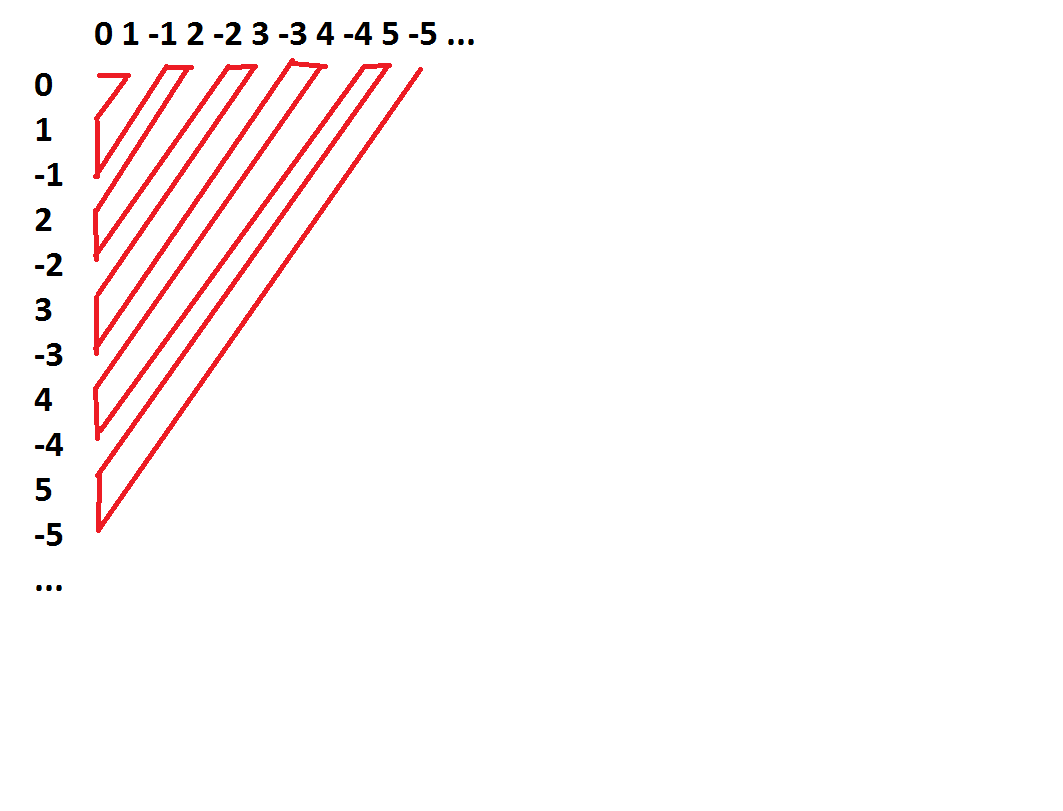
\includegraphics[scale=.5]{counting.png}
\newline
\newline
\textbf{Step: } Assume can count polynomials of degree $k$, show can count polynomials of degree $k+1$
\newline
\newline
Consider a polynomial of degree $k+1$. We write this as $\sum\limits_{i=0}^{k+1} c_i\cdot x^i = c_{k+1} x^i + \sum\limits_{i=0}^{k} c_k x^i$. Thus we have a number of choices for $c_{k+1}$ and the degree $k$ polynomial to the right of it. But we can count the number of polynomials of degree $k$. Namely, we can list start listing off $p_1, p_2, ...$ and so on forever and eventually get to any polynomial we want. Similarly, because $c_{k+1}$ is integral, we can list off $0, 1, -1, ...$ as above. Thus, using the exact same scheme as in the base, we can put the degree $k$ polynomials at the top of a box and put the values of $c_{k+1}$ as above at the side of a box, draw diagonally, and we will eventually reach any polynomial we want. Thus, the polynomials of degree $k+1$ are countable assuming the polynomials of degree $k$ are.
\newline
\newline
Having shown the statement holds for the base and the step, we conclude that all polynomials with fixed degree $k$ are countable.
\newline
\newline
2. Prove that the set of all such polynomials, where the degree $k$ ranges over the nonnegative integers, is countable.
\newline
\newline
I'm going to draw another shitty picture for you. I hope you like it:
\newline
\newline
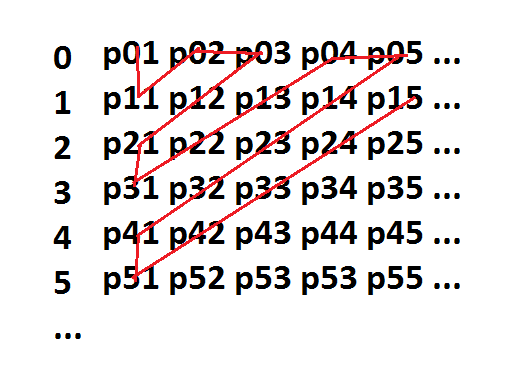
\includegraphics[scale=.5]{counting2.png}
\newline
\newline
Because $k$ is countable, we can put it on the left side of the box. Then, because each polynomial of degree $k$ is countable, we can impose an ordering over all polynomials of degree $k$, write them down in that order in the row corresponding to their degree, and then draw through them just like we did before. In the drawing $p_{ij}$ indicates polynomial $j$ in the set of polynomials of degree $i$. Thus, the set of all polynomials with degree $k \geq 0$ is countable.
% End sol%

\pagebreak{}

\thispagestyle{empty}

\begin{tabular*}{1\textwidth}{@{\extracolsep{\fill}}lr}
\textbf{ID:} 03 & \textbf{Josh Chen \#1:} Last Name, First Name\tabularnewline
\textbf{Name:} Al-Naji, Nader & \textbf{Collaborator \#2:} Last Name, First Name\tabularnewline
\hline 
\end{tabular*}

\medskip{}


\begin{center}
\begin{Large}\textbf{Solution to HW 11, Problem 2}\end{Large}
\par\end{center}

\begin{center}
\begin{large}\textbf{COS 340 - Spring 2012}\end{large}
\par\end{center}

\bigskip{}


% Begin sol%
For each of the following languages, determine whether they are decidable or recognizable, accompanied by proofs. Let $M$ be a Turing maching and $<M>$ be its encoding. Let $L(M)$ denote the language denoted by the Turing machine $M$.
\newline
\newline
1. $L_1 = {<M> : L(M) \mbox{is finite}}$
\newline
\newline
We start by showing that if $L_1$ were decidable, then $A_{tm}$ would also be decidable, a contradiction. $L_1$ is the set of Turing machines that accept a language of infinite size. We can define a Turing machine $M$ and arbitrary input $W$ for $M$. We now define a Turing machine $R$ to be run on inputs $x$ as follows:
\newline
\newline
$R(x):$ \newline
\indent if ($M$ accepts $W$)\newline
\indent\indent accept\newline
\indent else\newline
\indent\indent reject\newline
\newline
\newline
It should be clear that $L(R)$ is infinite if $M$ accepts $W$ since, in that case, $R$ would accept all strings. It should also be clear that if $L(R) = \emptyset$ if $M$ does not accept $W$ since in this case $R$ would reject all strings.
\newline
\newline
We can now use $R$ to construct two new machines $Q$ and $S$ that we can use to decide $L_1$ and $A_{tm}$ such that $Q$ accepts if and only if $S$ accepts. A decider for $<R>$ must accept an input $<R>$ if and only if $L(R)$ is infinite. We can construct $Q$ by letting $Q$ accept $<R>$ if and only if $R$ accepts. We can do the same for $S$ letting $S$ accept if and only if $M$ accepts $W$, making it a decider for $A_{tm}$. Since we defined $R$ to accept if and only if $M$ accepts $W$, this means that $Q$ accepts if and only if $S$ accepts, which means that if there existed a decider for $L_1$, then we could use it to decide $A_{tm}$, a contradiction.
\newline
\newline
We follow a similar proof as above and again show that if $L_1$ were recognizable, then $A_{tm}$ would be as well, a contradiction. Assume that there exists a Turing machine $Q$ that recognizes $L_1$. That is, assume there exists a Turing machine that accepts a string if and only if it is in $L_1$. Consider the following enumerator $E$ that runs on a Turing machine $M$ and takes input $W$ and simply alternates between enumerating and printing all strings in $\Sigma *$ and running $M$ on $W$. Note that $E$ does not accept until $M$ accepts $W$:
\newline
\newline
$E(x)$\newline
\indent initialize string to $0$\newline
\indent loop forever\newline
\indent\indent print string\newline
\indent \indent Run $M(W)$ for one step\newline
\indent\indent if $M$ accepts $W$\newline
\indent\indent\indent accept\newline
\indent\indent if $M$ rejects $W$\newline
\indent\indent\indent loop forever only printing and stepping string each time \newline
\indent\indent step string by one\newline
\newline
\newline
It should be clear that this machine accepts if $M$ accepts $W$ and prints forever if $M$ rejects $W$ or if $M$ doesn't halt. Now consider a machine $R$ that, given an input $x$ will run $E$ until the string it is printing is equal to $x$. It should be clear that if $M$ does not accept $W$ then $E$ will generate strings indefinitely and therefore $R$ will eventually hit $x$ and accept, making $L(R)$ accept on all strings, making $L(R)$ infinite. On the other hand, if $M$ accepts $W$ then $E$ will stop after some finite time and so $L(R)$ will be finite. The proof from here follows similarly to part one. Let $Q$ be a recognizer for $L_1$ that accepts an input $<R>$ if and only if $R$ accepts all strings and, therefore, if and only if $M$ does not accept $W$. Define the recognizer for $A_{tm}$ that accepts an input $<M, W>$ if and only if $M$ does not accept $W$ to be $S$. Since the criteria for acceptance are the same for $Q$ and $S$, that is, since $Q$ recognizes $<R>$ if and only if $S$ recognizes $<M, W>$, if there existed such a recognizer for $L_1$ $Q$, then we can use $Q$ to recognize $A_{tm}$ as well by defining an enumerator and a machine such as $R$ and running $<R>$ on Q. Thus we have a contradiction.
\newline
\newline
Thus we have shown that $L_1$ is neither recognizable nor decidable.
\newline
\newline
2. $L_2 = {<M>: L(M) \mbox{is uncountable}}$ \newline\newline
Since we showed in the notes that $\Sigma *$ is countable and that the input of any Turing machine must be a string $s \in \Sigma *$, it must be the case that $L(M) \subseteq \Sigma *$ and, since there exist no Turing machines with uncountable $L(M)$, $L_2$ must be empty. Thus, we can construct a recognizer and a decider for $L_2$ by simply constructing a Turing Machine that rejects all inputs. Thus, since we can do this, $L_2$ is both decidable and recognizable. 
% End sol%

\pagebreak{}
\thispagestyle{empty}

\begin{tabular*}{1\textwidth}{@{\extracolsep{\fill}}lr}
\textbf{ID:} 03 & \textbf{Collaborator \#1:} Last Name, First Name\tabularnewline
\textbf{Name:} Al-Naji, Nader & \textbf{Collaborator \#2:} Last Name, First Name\tabularnewline
\hline 
\end{tabular*}

\medskip{}


\begin{center}
\begin{Large}\textbf{Solution to HW 11, Problem 3}\end{Large}
\par\end{center}

\begin{center}
\begin{large}\textbf{COS 340 - Spring 2012}\end{large}
\par\end{center}

\bigskip{}


% Begin sol%
Suppose that someone gives you a black-box algorithm $A$ that takes an undirected graph $G = (V, E)$, and a number $k$, and behaves as follows:
\newline
If $G$ is not connected, it simply returns ``$G$ is not connected.''\newline
If $G$ is connected and has an independent set of size at least $k$, it returns ``yes''\newline
If $G$ is connected and does not have an independent set of size at least $k$, it returns ``no''\newline
\newline
Suppose that the algorithm $A$ runs in time polynomial in the size of $G$ and $k$. Show how, using calls to $A$, you could then solve the Independent Set Problem in polynomial time. That is show how you could answer the question: Given an arbitrary undirected graph $G$, and a number $k$, does $G$ contain an independent set of size at least $k$?
\newline
\newline
The problem with this algorithm is that it tells us nothing about graphs that are not connected. To remedy this, we consider adding a new vertex to connect the original graph $G$. We consider adding a vertex, connecting it to every vertex in $G$, and showing that adding such a vertex can not possibly have an effect on the size of the largest independent set. First, note that if we add such a vertex and can verify that the size of the maximum independent set does not change, then we can use the above algorithm directly on our augmented graph to answer the question about the original graph, since the answer to the question will be the same. Further, since adding such a vertex is only an $O(V)$ operation, if we add this vertex and make a single call to the algorithm, we solve the problem in time polynomial in $k$ and $G$ as specified. We now consider why adding such a vertex cannot possibly affect the size of the maximum independent set. First, consider what happens if our new vertex is in the maximum independent set. If this is the case, then no other vertices can be in the maximum independent set since the new vertex is connected to all of them. So the size of the maximum independent set if we include this vertex is exactly one. Now consider the case where this vertex is not in the maximum independent set. If our graph originally had a maximum independent set of size $k$, then, because this new vertex did not introduce any new edges between any of the original vertices in $G$, the size of the maximum independent set if we don't allow this vertex to be in it is again equal to $k$. Thus, if the size of the maximum independent set was one originally, then one of the two cases could occur but neither would change the size of the maximum independent set and, therefore, neither could change the algorithm's answer. And if the size of the maximum independent set was originally larger than one, then this vertex will simply not be included (since including it would decrease the size of the set) and the size of the maximum independent set will remain unchanged, again not affecting the outcome of the algorithm. Thus, connecting the graph with such a vertex allows us to answer the question about the original graph, without loss of generality, with a single call to the algorithm and an $O(V)$ cost increase, thus introducing a poly-time algorithm to compute the maximum independent set using calls to $A$. Note that the minimum size of the maximum independent set is one since we assume no self loops.
% End sol%

\pagebreak{}

\thispagestyle{empty}

\begin{tabular*}{1\textwidth}{@{\extracolsep{\fill}}lr}
\textbf{ID:} 03 & \textbf{Collaborator \#1:} Last Name, First Name\tabularnewline
\textbf{Name:} Al-Naji, Nader & \textbf{Collaborator \#2:} Last Name, First Name\tabularnewline
\hline 
\end{tabular*}

\medskip{}


\begin{center}
\begin{Large}\textbf{Solution to HW 11, Problem 4}\end{Large}
\par\end{center}

\begin{center}
\begin{large}\textbf{COS 340 - Spring 2012}\end{large}
\par\end{center}

\bigskip{}


% Begin sol%
1. Suppose we implement a secret sharing scheme using polynomials. The secret $s$ is an integer in {0, 1, ..., 10}. We will work modulo 11. We pick a degree two polynomial $f(x) = a_0 + a_1 x + a_2 x^2 (mod 11)$ where $a_0 = s$ and $a_1, a_2$ are chosen randomly from {0, 1, ..., 10}. Given that $f(1) = 2, f(2) = 4, f(3) = 8$, find the polynomial $f(x)$.
\newline
\newline
We have the points $(1, 2), (2, 4), and (3, 8)$. We use Lagrange interpolation to construct three polynomials that are $1$ when $f(x) = 1, 2, 3$ and zero otherwise, multiply them by their respective $y$ values, and then add them together. The resulting polynomial will be $y_i$ for its corresponding $x$ since the other polynomials will be zero by construction and thus the polynomial will fit the three points. 
\newline
\newline
$\nabla_1(x) = \frac{(x-2)(x-3)}{(1-2)(1-3)} = \frac{(x-2)(x-3)}{2} = 6(x-2)(x-3) (mod 11)$\newline
$\nabla_2(x) = \frac{(x-1)(x-3)}{(2-1)(2-3)} = \frac{(x-1)(x-3)}{-1} = -(x-1)(x-3) (mod 11)$\newline
$\nabla_3(x) = \frac{(x-1)(x-2)}{(3-1)(3-2)} = \frac{(x-1)(x-2)}{2} = 6(x-1)(x-2) (mod 11)$\newline
$\rightarrow p(x) = 2 \nabla_1(x) + 4 \nabla_2(x) + 8 \nabla_3(x) = x^2 + 10x + 2 (mod 11)$.
\newline
\newline
Consider a polynomial $p(x) = \sum\limits_{i=0}^{n} a_i x^i$ where the coefficients are non-negative integers. Amazingly, it is possible to figure out the coefficients $a_i$ by asking for the values of $p(x)$ at only two carefully chosen points. First, we ask for $p(1)$. Suppose $p(1) = r$. Next, we ask for $p(r+1)$. Show how you can determine $p(x)$ completely from this information.
\newline
\newline
We have $r = p(1) = \sum\limits_{i=0}^{n} a_i \rightarrow r \geq a_i \mbox{ } \forall \mbox{ } i$ on domain since the $a_i$ are nonnegative. Let $q = p(r+1) = a_n (r+1)^n + ... + a_0 (r+1)^0$. From the fact that $r \geq a_i \mbox{ } \forall \mbox{ } i$, we have that $r+1 > a_i \mbox{ } \forall \mbox{ } i$. This means that we can interpret $p(r+1)$ as the $base_{r+1}$ encoding of $q$. So if we can convert $q = p(r+1)$ into $base_{r+1}$, then $q$ will be an $n$ digit number and, further, the $i_{th}$ digit of $q$ will uniquely identify $a_i$ for all $i$ in the domain. Again, this is valid only because $0 \leq a_i < r+1 \mbox{ } \forall \mbox{ } i$ on the domain. 

% End sol%

\pagebreak{}

\end{document}
